%%% MATH110-PS00A-Solutions.tex --- 
%% 
%% Filename: MATH110-PS00A-Solutions.tex
%% Description: 
%% Author: U-ORONYA\edwar
%% Maintainer: 
%% Created: Sun Jan 29 23:40:40 2023 (-0600)
%% Version: 
%% Package-Requires: ()
%% Last-Updated: Sun Jan 29 23:41:49 2023 (-0600)
%%           By: U-ORONYA\edwar
%%     Update #: 2
%% URL: 
%% Doc URL: 
%% Keywords: 
%% Compatibility: 
%% 
%%%%%%%%%%%%%%%%%%%%%%%%%%%%%%%%%%%%%%%%%%%%%%%%%%%%%%%%%%%%%%%%%%%%%%
%% 
%%% Commentary: 
%% 
%% 
%% 
%%%%%%%%%%%%%%%%%%%%%%%%%%%%%%%%%%%%%%%%%%%%%%%%%%%%%%%%%%%%%%%%%%%%%%
%% 
%%% Change Log:
%% 
%% 
%%%%%%%%%%%%%%%%%%%%%%%%%%%%%%%%%%%%%%%%%%%%%%%%%%%%%%%%%%%%%%%%%%%%%%
%%
%% Copyright (C) 2023 Edward Doolittle
%% 
%%%%%%%%%%%%%%%%%%%%%%%%%%%%%%%%%%%%%%%%%%%%%%%%%%%%%%%%%%%%%%%%%%%%%%
%% 
%%% Code:


\documentclass{article}
\usepackage{amsmath}
\usepackage{fullpage}
%\usepackage{graphicx}
\usepackage{tikz}
\usetikzlibrary{calc}
%\usepackage{pgfmath}
\usepackage[aux]{rerunfilecheck}

% Macros for MATH 110 course dates

\newcommand{\commonTheme}{metropolis}
\newcommand{\commonColorTheme}{metropolis}

\newcommand{\commonAuthor}{Edward Doolittle}
\newcommand{\commonInstitute}{Department of Indigenous Knowledge and
  Science \\ First Nations University of Canada}
\newcommand{\commonCourse}{MATH 110 Calculus I}
\newcommand{\commonTerm}{202510}
\newcommand{\commonDate}{January 6, 2025}

% Review Material

% Lab 0
\newcommand{\commonEventNegativeOne}{LabNegativeOne}
\newcommand{\commonDateLabNegativeOne}{Monday, January 6, 2025}
\newcommand{\commonTitleLabNegativeOne}{MATH 110 Lab 0}
\newcommand{\commonSubtitleLabNegativeOne}{No Lab; Course Opens}

% Section 001
\newcommand{\commonEventZeroZeroOne}{ZeroZeroOne}
\newcommand{\commonDateZeroZeroOne}{Tuesday, January 7, 2025}
\newcommand{\commonTitleZeroZeroOne}{MATH 110 Review 0.1}
\newcommand{\commonSubtitleZeroZeroOne}{Review of Algebra}
\newcommand{\commonPSTitleZeroZeroOne}{MATH 110 Review Problem Set 0.1}

% Section 00A
\newcommand{\commonEventZeroZeroA}{ZeroZeroA}
\newcommand{\commonDateZeroZeroA}{Tuesday, January 7, 2025}
\newcommand{\commonTitleZeroZeroA}{MATH 110 Review 0.A}
\newcommand{\commonSubtitleZeroZeroA}{Review of Inequalities and
  Absolute Values}
\newcommand{\commonPSTitleZeroZeroA}{MATH 110 Review Problem Set 0.A}

% Section 00B
\newcommand{\commonEventZeroZeroB}{ZeroZeroB}
\newcommand{\commonDateZeroZeroB}{Tuesday, January 7, 2025}
\newcommand{\commonTitleZeroZeroB}{MATH 110 Review 0.B}
\newcommand{\commonSubtitleZeroZeroB}{Review of Coordinate Geometry
  and Lines}
\newcommand{\commonPSTitleZeroZeroB}{MATH 110 Review Problem Set 0.B}

% Section 00C
\newcommand{\commonEventZeroZeroC}{ZeroZeroC}
\newcommand{\commonDateZeroZeroC}{Thursday, January 9, 2025}
\newcommand{\commonTitleZeroZeroC}{MATH 110 Review 0.C}
\newcommand{\commonSubtitleZeroZeroC}{Review of Graphs of Second
  Degree Equations}
\newcommand{\commonPSTitleZeroZeroC}{MATH 110 Review Problem Set 0.C}

% Section 00D
\newcommand{\commonEventZeroZeroD}{ZeroZeroD}
\newcommand{\commonDateZeroZeroD}{Thursday, January 9, 2025}
\newcommand{\commonTitleZeroZeroD}{MATH 110 Review 0.D}
\newcommand{\commonSubtitleZeroZeroD}{Review of Trigonometry}
\newcommand{\commonPSTitleZeroZeroD}{MATH 110 Review Problem Set 0.D}

% Section 011
\newcommand{\commonEventZeroOneOne}{ZeroOneOne}
\newcommand{\commonDateZeroOneOne}{Thursday, January 9, 2025}
\newcommand{\commonTitleZeroOneOne}{MATH 110 Review 1.1}
\newcommand{\commonSubtitleZeroOneOne}{Review of Functions}
\newcommand{\commonPSTitleZeroOneOne}{MATH 110 Review Problem Set 1.1}


% Main Course

% Lab 1
\newcommand{\commonEventZero}{LabZero}
\newcommand{\commonDateLabZero}{Monday, January 13, 2025}
\newcommand{\commonTitleLabZero}{MATH 110 Lab 1}
\newcommand{\commonSubtitleLabZero}{Quiz 0: STACK, Onboarding}

% Section 1.4
\newcommand{\commonEventOne}{ZeroOneFour}
\newcommand{\commonDateZeroOneFour}{Tuesday, January 14, 2025}
\newcommand{\commonTitleZeroOneFour}{MATH 110 Lecture 1.4}
\newcommand{\commonSubtitleZeroOneFour}{The Tangent and Velocity Problems}
\newcommand{\commonPSTitleZeroOneFour}{MATH 110 Problem Set 1.4}

% Section 1.5
\newcommand{\commonEventTwo}{ZeroOneFive}
\newcommand{\commonDateZeroOneFive}{Thursday, January 16, 2025}
\newcommand{\commonTitleZeroOneFive}{MATH 110 Lecture 1.5}
\newcommand{\commonSubtitleZeroOneFive}{The Limit of a Function}
\newcommand{\commonPSTitleZeroOneFive}{MATH 110 Problem Set 1.5}

% Lab 2
\newcommand{\commonEventThree}{LabOne}
\newcommand{\commonDateLabOne}{Monday, January 20, 2025}
\newcommand{\commonTitleLabOne}{MATH 110 Lab 2}
\newcommand{\commonSubtitleLabOne}{Quiz 1: Review}

% Section 1.6
\newcommand{\commonEventFour}{ZeroOneSix}
\newcommand{\commonDateZeroOneSix}{Tuesday, January 21, 2025}
\newcommand{\commonTitleZeroOneSix}{MATH 110 Lecture 1.6}
\newcommand{\commonSubtitleZeroOneSix}{Calculating Limits Using the Limit Laws}
\newcommand{\commonPSTitleZeroOneSix}{MATH 110 Problem Set 1.6}

% Section 1.7
\newcommand{\commonEventFive}{ZeroOneSeven}
\newcommand{\commonDateZeroOneSeven}{(Not covered)}
\newcommand{\commonTitleZeroOneSeven}{MATH 110 Lecture 1.7}
\newcommand{\commonSubtitleZeroOneSeven}{The Precise Definition of a Limit}
\newcommand{\commonPSTitleZeroOneSeven}{MATH 110 Problem Set 1.7}

% Section 1.8
\newcommand{\commonEventSix}{ZeroOneEight}
\newcommand{\commonDateZeroOneEight}{Thursday, January 23, 2025}
\newcommand{\commonTitleZeroOneEight}{MATH 110 Lecture 1.8}
\newcommand{\commonSubtitleZeroOneEight}{Continuity}
\newcommand{\commonPSTitleZeroOneEight}{MATH 110 Problem Set 1.8}

% Lab 3
\newcommand{\commonEventSeven}{LabTwo}
\newcommand{\commonDateLabTwo}{Monday, January 27, 2025}
\newcommand{\commonTitleLabTwo}{MATH 110 Lab 3}
\newcommand{\commonSubtitleLabTwo}{Quiz 2: Sections 1.4, 1.5}

% Section 2.1
\newcommand{\commonEventEight}{ZeroTwoOne}
\newcommand{\commonDateZeroTwoOne}{Tuesday, January 28, 2025}
\newcommand{\commonTitleZeroTwoOne}{MATH 110 Lecture 2.1}
\newcommand{\commonSubtitleZeroTwoOne}{Derivatives and Rates of Change}
\newcommand{\commonPSTitleZeroTwoOne}{MATH 110 Problem Set 2.1}

% Section 2.2
\newcommand{\commonEventNine}{ZeroTwoTwo}
\newcommand{\commonDateZeroTwoTwo}{Thursday, January 30, 2025}
\newcommand{\commonTitleZeroTwoTwo}{MATH 110 Lecture 2.2}
\newcommand{\commonSubtitleZeroTwoTwo}{The Derivative as a Function}
\newcommand{\commonPSTitleZeroTwoTwo}{MATH 110 Problem Set 2.2}

% Lab 4
\newcommand{\commonEventTen}{LabThree}
\newcommand{\commonDateMTOne}{Monday, February 3, 2025} 
\newcommand{\commonDateLabThree}{Monday, February 3, 2025}
\newcommand{\commonTitleLabThree}{MATH 110 Lab 4}
\newcommand{\commonSubtitleLabThree}{Midterm: Review, Chapter 1}

% Section 2.3
\newcommand{\commonEventEleven}{ZeroTwoThree}
\newcommand{\commonDateZeroTwoThree}{Tuesday, February 4, 2025}
\newcommand{\commonTitleZeroTwoThree}{MATH 110 Lecture 2.3}
\newcommand{\commonSubtitleZeroTwoThree}{Differentiation Formulas}
\newcommand{\commonPSTitleZeroTwoThree}{MATH 110 Problem Set 2.3}

% Section 2.4
\newcommand{\commonEventTwelve}{ZeroTwoFour}
\newcommand{\commonDateZeroTwoFour}{Thursday, February 6, 2025}
\newcommand{\commonTitleZeroTwoFour}{MATH 110 Lecture 2.4}
\newcommand{\commonSubtitleZeroTwoFour}{Derivatives of Trigonometric Functions}
\newcommand{\commonPSTitleZeroTwoFour}{MATH 110 Problem Set 2.4}

% Lab 5
\newcommand{\commonEventThirteen}{LabFour}
\newcommand{\commonDateLabFour}{Monday, February 10, 2025}
\newcommand{\commonTitleLabFour}{MATH 110 Lab 5}
\newcommand{\commonSubtitleLabFour}{Quiz 3: Sections 2.1, 2.2}

% Section 2.5
\newcommand{\commonEventFourteen}{ZeroTwoFive}
\newcommand{\commonDateZeroTwoFive}{Tuesday, February 11, 2025}
\newcommand{\commonTitleZeroTwoFive}{MATH 110 Lecture 2.5}
\newcommand{\commonSubtitleZeroTwoFive}{The Chain Rule}
\newcommand{\commonPSTitleZeroTwoFive}{MATH 110 Problem Set 2.5}

% Section 2.6
\newcommand{\commonEventFifteen}{ZeroTwoSix}
\newcommand{\commonDateZeroTwoSix}{Thursday, February 13, 2025}
\newcommand{\commonTitleZeroTwoSix}{MATH 110 Lecture 2.6}
\newcommand{\commonSubtitleZeroTwoSix}{Implicit Differentiation}
\newcommand{\commonPSTitleZeroTwoSix}{MATH 110 Problem Set 2.6}

% Lab 6
\newcommand{\commonEventSixteen}{LabFive}
\newcommand{\commonDateLabFive}{Monday, February 24, 2025}
\newcommand{\commonTitleLabFive}{MATH 110 Lab 6}
\newcommand{\commonSubtitleLabFive}{Quiz 4: Sections 2.3, 2.4}

% Section 2.7
\newcommand{\commonEventSeventeen}{ZeroTwoSeven}
\newcommand{\commonDateZeroTwoSeven}{Tuesday, February 25, 2025}
\newcommand{\commonTitleZeroTwoSeven}{MATH 110 Lecture 2.7}
\newcommand{\commonSubtitleZeroTwoSeven}{Rates of Change in the
  Natural and Social Sciences}
\newcommand{\commonPSTitleZeroTwoSeven}{MATH 110 Problem Set 2.7}

% Section 2.8
\newcommand{\commonEventEighteen}{ZeroTwoEight}
\newcommand{\commonDateZeroTwoEight}{Thursday, February 27, 2025}
\newcommand{\commonTitleZeroTwoEight}{MATH 110 Lecture 2.8}
\newcommand{\commonSubtitleZeroTwoEight}{Related Rates}
\newcommand{\commonPSTitleZeroTwoEight}{MATH 110 Problem Set 2.8}

% Lab 7
\newcommand{\commonEventNineteen}{LabSix}
\newcommand{\commonDateLabSix}{Monday, March 3, 2025}
\newcommand{\commonTitleLabSix}{MATH 110 Lab 7}
\newcommand{\commonSubtitleLabSix}{Quiz 5: Sections 2.5, 2.6}

% Section 3.1
\newcommand{\commonEventTwenty}{ZeroThreeOne}
\newcommand{\commonDateZeroThreeOne}{Tuesday, March 4, 2025}
\newcommand{\commonTitleZeroThreeOne}{MATH 110 Lecture 3.1}
\newcommand{\commonSubtitleZeroThreeOne}{Maximum and Minimum Values}
\newcommand{\commonPSTitleZeroThreeOne}{MATH 11 Problem Set 3.1}

% Section 3.2
\newcommand{\commonEventTwentyOne}{ZeroThreeTwo}
\newcommand{\commonDateZeroThreeTwo}{Thursday, March 6, 2025}
\newcommand{\commonTitleZeroThreeTwo}{MATH 110 Lecture 3.2}
\newcommand{\commonSubtitleZeroThreeTwo}{The Mean Value Theorem}
\newcommand{\commonPSTitleZeroThreeTwo}{MATH 110 Problem Set 3.2}

% Lab 8
\newcommand{\commonEventTwentyTwo}{LabSeven}
\newcommand{\commonDateMTTwo}{Monday, March 10, 2025}
\newcommand{\commonDateLabSeven}{Monday, March 10, 2025}
\newcommand{\commonTitleLabSeven}{MATH 110 Lab 8}
\newcommand{\commonSubtitleLabSeven}{Midterm: Chapter 2}

% Section 3.3
\newcommand{\commonEventTwentyThree}{ZeroThreeThree}
\newcommand{\commonDateZeroThreeThree}{Tuesday, March 11, 2025}
\newcommand{\commonTitleZeroThreeThree}{MATH 110 Lecture 3.3}
\newcommand{\commonSubtitleZeroThreeThree}{How Derivatives Affect the
  Shape of a Graph}
\newcommand{\commonPSTitleZeroThreeThree}{MATH 110 Problem Set 3.3}

% Section 3.4
\newcommand{\commonEventTwentyFour}{ZeroThreeFour}
\newcommand{\commonDateZeroThreeFour}{Thursday, March 13, 2025}
\newcommand{\commonTitleZeroThreeFour}{MATH 110 Lecture 3.4}
\newcommand{\commonSubtitleZeroThreeFour}{Limits at Infinity;
  Horizontal Asymptotes}
\newcommand{\commonPSTitleZeroThreeFour}{MATH 110 Problem Set 3.4}

% Lab 9
\newcommand{\commonEventTwentyFive}{LabEight}
\newcommand{\commonDateLabEight}{Monday, March 17, 2025}
\newcommand{\commonTitleLabEight}{MATH 110 Lab 9}
\newcommand{\commonSubtitleLabEight}{Quiz 6: Sections 3.1, 3.2}

% Section 3.5
\newcommand{\commonEventTwentySix}{ZeroThreeFive}
\newcommand{\commonDateZeroThreeFive}{Tuesday, March 18, 2025}
\newcommand{\commonTitleZeroThreeFive}{MATH 110 Lecture 3.5}
\newcommand{\commonSubtitleZeroThreeFive}{Summary of Curve Sketching}
\newcommand{\commonPSTitleZeroThreeFive}{MATH 110 Problem Set 3.5}

% Section 3.7
\newcommand{\commonEventTwentySeven}{ZeroThreeSeven}
\newcommand{\commonDateZeroThreeSeven}{Thursday, March 20, 2025}
\newcommand{\commonTitleZeroThreeSeven}{MATH 110 Lecture 3.7}
\newcommand{\commonSubtitleZeroThreeSeven}{Optimization Problems}
\newcommand{\commonPSTitleZeroThreeSeven}{MATH 110 Problem Set 3.7}

% Lab 10
\newcommand{\commonEventTwentyEight}{LabNine}
\newcommand{\commonDateLabNine}{Monday, March 24, 2025}
\newcommand{\commonTitleLabNine}{MATH 110 Lab 10}
\newcommand{\commonSubtitleLabNine}{Quiz 7: Sections 3.3, 3.4}

% Section 4.1
\newcommand{\commonEventTwentyNine}{ZeroFourOne}
\newcommand{\commonDateZeroFourOne}{Tuesday, March 25, 2025}
\newcommand{\commonTitleZeroFourOne}{MATH 110 Lecture 4.1}
\newcommand{\commonSubtitleZeroFourOne}{Areas and Distances}
\newcommand{\commonPSTitleZeroFourOne}{MATH 110 Problem Set 4.1}

% Section 4.2
\newcommand{\commonEventThirty}{ZeroFourTwo}
\newcommand{\commonDateZeroFourTwo}{Thursday, March 27, 2025}
\newcommand{\commonTitleZeroFourTwo}{MATH 110 Lecture 4.2}
\newcommand{\commonSubtitleZeroFourTwo}{The Definite Integral}
\newcommand{\commonPSTitleZeroFourTwo}{MATH 110 Problem Set 4.2}

% Lab 11
\newcommand{\commonEventThirtyOne}{LabTen}
\newcommand{\commonDateLabTen}{Monday, March 31, 2025}
\newcommand{\commonTitleLabTen}{MATH 110 Lab 11}
\newcommand{\commonSubtitleLabTen}{Quiz 8: Sections 3.5, 3.7}

% Section 4.3
\newcommand{\commonEventThirtyTwo}{ZeroFourThree}
\newcommand{\commonDateZeroFourThree}{Tuesday, April 1, 2025}
\newcommand{\commonTitleZeroFourThree}{MATH 110 Lecture 4.3}
\newcommand{\commonSubtitleZeroFourThree}{The Fundamental Theorem of Calculus}
\newcommand{\commonPSTitleZeroFourThree}{MATH 110 Problem Set 4.3}

% Section 4.4
\newcommand{\commonEventThirtyThree}{ZeroFourFour}
\newcommand{\commonDateZeroFourFour}{Thursday, April 3, 2025}
\newcommand{\commonTitleZeroFourFour}{MATH 110 Lecture 4.4}
\newcommand{\commonSubtitleZeroFourFour}{Indefinite Integrals and the
  Net Change Theorem}
\newcommand{\commonPSTitleZeroFourFour}{MATH 110 Problem Set 4.4}

% Lab 12
\newcommand{\commonEventThirtyFour}{LabEleven}
\newcommand{\commonDateLabEleven}{Monday, April 7, 2025}
\newcommand{\commonTitleLabEleven}{MATH 110 Lab 12}
\newcommand{\commonSubtitleLabEleven}{Quiz 9: Sections 4.1, 4.2}

% Section 4.5
\newcommand{\commonEventThirtyFive}{ZeroFourFive}
\newcommand{\commonDateZeroFourFive}{Tuesday, April 8, 2025}
\newcommand{\commonTitleZeroFourFive}{MATH 110 Lecture 4.5}
\newcommand{\commonSubtitleZeroFourFive}{The Substitution Rule}
\newcommand{\commonPSTitleZeroFourFive}{MATH 110 Problem Set 4.5}

% Section 5.1
\newcommand{\commonEventThirtySix}{ZeroFiveOne}
\newcommand{\commonDateZeroFiveOne}{Thursday, April 10, 2025}
\newcommand{\commonTitleZeroFiveOne}{MATH 110 Lecture 5.1}
\newcommand{\commonSubtitleZeroFiveOne}{Areas Between Curves}
\newcommand{\commonPSTitleZeroFiveOne}{MATH 110 Problem Set 5.1}

% Lab 13
\newcommand{\commonEventThirtySeven}{LabTwelve}
\newcommand{\commonDateLabTwelve}{Monday, April 14, 2025}
\newcommand{\commonTitleLabTwelve}{MATH 110 Review Lab}
\newcommand{\commonSubtitleLabTwelve}{Bonus Quiz 10: Sections 4.3, 4.4}

% Final Class
\newcommand{\commonEventThirtyEight}{FinalClass}
\newcommand{\commonDateFinalClass}{Tuesday, April 15, 2025}
\newcommand{\commonTitleFinalClass}{MATH 110 Review Class}
\newcommand{\commonSubtitleFinalClass}{Answer Questions, Review for Exam}

% Final Exam
\newcommand{\commonEventThirtyNine}{Final}
\newcommand{\commonDateFinal}{Thursday, April 22, 2025}
\newcommand{\commonTitleFinal}{MATH 110 Final Exam}
\newcommand{\commonSubtitleFinal}{Comprehensive Exam: All Sections}

% Orphaned -- no longer part of the course

% Section 2.9
\newcommand{\commonDateZeroTwoNine}{Not part of the course}
\newcommand{\commonTitleZeroTwoNine}{MATH 110 Lecture 2.9}
\newcommand{\commonSubtitleZeroTwoNine}{Linear Approximations and Differentials}
\newcommand{\commonPSTitleZeroTwoNine}{MATH 110 Problem Set 2.9}


% % Introduction
% \newcommand{\commonEventOneDate}{Wednesday, September 8, 2010}
% \newcommand{\commonEventOneDesc}{Introduction to the Course}
% \newcommand{\commonDateZeroZeroZero}{September 8, 2010}
% \newcommand{\commonTitleZeroZeroZero}{MATH 104 Introduction}
% \newcommand{\commonSubtitleZeroZeroZero}{Outline of the Course}

% % Lecture 1
% \newcommand{\commonEventTwoDate}{Friday, September 10, 2010}
% \newcommand{\commonEventTwoDesc}{Lecture 1: Algebra}
% \newcommand{\commonDateZeroZeroOne}{September 10, 2010}
% \newcommand{\commonTitleZeroZeroOne}{MATH 104 Lecture 1}
% \newcommand{\commonSubtitleZeroZeroOne}{Review of Algebra}
% % associated evaluation ... factor this out?
% \newcommand{\commonPSTitleZeroZeroOne}{MATH 104 Problem Set 1}
% \newcommand{\commonEvalZeroZeroOne}{Quiz 1}
% \newcommand{\commonEvalDateZeroZeroOne}{Wednesday, September 15, 2010}

% % Lecture 2
% \newcommand{\commonEventThreeDate}{Monday, September 13, 2010}
% \newcommand{\commonEventThreeDesc}{Lecture 2: Appendix A}
% \newcommand{\commonDateZeroZeroA}{September 13, 2010}
% \newcommand{\commonTitleZeroZeroA}{MATH 104 Lecture 2}
% \newcommand{\commonSubtitleZeroZeroA}{Appendix A: Numbers, Inequalities, 
%   and Absolute Values}
% % associated evaluation ... factor this out?
% \newcommand{\commonPSTitleZeroZeroA}{MATH 104 Problem Set 2}
% \newcommand{\commonEvalZeroZeroA}{Quiz 2}
% \newcommand{\commonEvalDateZeroZeroA}{Wednesday, September 22, 2010}

% % Review 1
% \newcommand{\commonEventFourDate}{Wednesday, September 15, 2010}
% \newcommand{\commonEventFourDesc}{Review 1: Review Algebra; Quiz 1; Review Appendix A}
% \newcommand{\commonDateRZeroOne}{September 15, 2010}
% \newcommand{\commonTitleRZeroOne}{MATH 104 Review 1}
% \newcommand{\commonSubtitleRZeroOne}{Review of Algebra, Appendix A}

% % Lecture 3
% \newcommand{\commonEventFiveDate}{Friday, September 17, 2010}
% \newcommand{\commonEventFiveDesc}{Lecture 3: Appendix B}
% \newcommand{\commonDateZeroZeroB}{September 17, 2010}
% \newcommand{\commonTitleZeroZeroB}{MATH 104 Lecture 3}
% \newcommand{\commonSubtitleZeroZeroB}{Appendix B: Coordinate Geometry and Lines}
% % associated evaluation ... factor this out?
% \newcommand{\commonPSTitleZeroZeroB}{MATH 104 Problem Set 3}
% \newcommand{\commonEvalZeroZeroB}{Quiz 2}
% \newcommand{\commonEvalDateZeroZeroB}{Wednesday, September 22, 2010}

% % Lecture 4
% \newcommand{\commonEventSixDate}{Monday, Sepbember 20, 2010}
% \newcommand{\commonEventSixDesc}{Lecture 4: Appendix C}
% \newcommand{\commonDateZeroZeroC}{September 20, 2010}
% \newcommand{\commonTitleZeroZeroC}{MATH 104 Lecture 4}
% \newcommand{\commonSubtitleZeroZeroC}{Appendix C: Graphs of Second-Degree Equations}
% % associated evaluation ... factor this out?
% \newcommand{\commonPSTitleZeroZeroC}{MATH 104 Problem Set 4}
% \newcommand{\commonEvalZeroZeroC}{Midterm 0}
% \newcommand{\commonEvalDateZeroZeroC}{Wednesday, September 29, 2010}

% % Review 2
% \newcommand{\commonEventSevenDate}{Wednesday, September 22, 2010}
% \newcommand{\commonEventSevenDesc}{Review 2: Review Appendix B; Quiz 2; Review Appendix C}
% \newcommand{\commonDateRZeroTwo}{September 22, 2010}
% \newcommand{\commonTitleRZeroTwo}{MATH 104 Review 2}
% \newcommand{\commonSubtitleRZeroTwo}{Review of Appendices B and C}

% % Lecture 5
% \newcommand{\commonEventEightDate}{Friday, September 24, 2010}
% \newcommand{\commonEventEightDesc}{Lecture 5: Appendix D}
% \newcommand{\commonDateZeroZeroD}{September 24, 2010}
% \newcommand{\commonTitleZeroZeroD}{MATH 104 Lecture 5}
% \newcommand{\commonSubtitleZeroZeroD}{Appendix D: Trigonometry}
% % associated evaluation ... factor this out?
% \newcommand{\commonPSTitleZeroZeroD}{MATH 104 Problem Set 5}
% \newcommand{\commonEvalZeroZeroD}{Midterm 0}
% \newcommand{\commonEvalDateZeroZeroD}{Wednesday, September 29, 2010}

% % Lecture 6
% \newcommand{\commonEventNineDate}{Monday, September 27, 2010}
% \newcommand{\commonEventNineDesc}{Lecture 6: Section 1.1}
% \newcommand{\commonDateZeroOneOne}{September 27, 2010}
% \newcommand{\commonTitleZeroOneOne}{MATH 104 Lecture 6}
% \newcommand{\commonSubtitleZeroOneOne}{Section 1.1: Four Ways to Represent a Function}
% % associated evaluation ... factor this out?
% \newcommand{\commonPSTitleZeroOneOne}{MATH 104 Problem Set 6}
% \newcommand{\commonEvalZeroOneOne}{Quiz 3}
% \newcommand{\commonEvalDateZeroOneOne}{Wednesday, October 6, 2010}

% % Review 3
% \newcommand{\commonEventTenDate}{Wednesday, September 29, 2010}
% \newcommand{\commonEventTenDesc}{Review 3: Review Appendix D; 
%   Self-Assessment Midterm 0}
% \newcommand{\commonDateRZeroThree}{September 29, 2010}
% \newcommand{\commonTitleRZeroThree}{MATH 104 Review 3}
% \newcommand{\commonSubtitleRZeroThree}{Review of Appendix D}

% % Lecture 7
% \newcommand{\commonEventElevenDate}{Friday, October 1, 2010}
% \newcommand{\commonEventElevenDesc}{Lecture 7: Section 1.2}
% \newcommand{\commonDateZeroOneTwo}{October 1, 2010}
% \newcommand{\commonTitleZeroOneTwo}{MATH 104 Lecture 7}
% \newcommand{\commonSubtitleZeroOneTwo}{Section 1.2: Mathematical Models: A Catalog of Essential Functions}
% % associated evaluation ... factor this out?
% \newcommand{\commonPSTitleZeroOneTwo}{MATH 104 Problem Set 7}
% \newcommand{\commonEvalZeroOneTwo}{Quiz 3}
% \newcommand{\commonEvalDateZeroOneTwo}{Wednesday, October 6, 2010}

% % Lecture 8
% \newcommand{\commonEventTwelveDate}{Monday, October 4, 2010}
% \newcommand{\commonEventTwelveDesc}{Lecture 8: Section 1.3}
% \newcommand{\commonDateZeroOneThree}{October 4, 2010}
% \newcommand{\commonTitleZeroOneThree}{MATH 104 Lecture 8}
% \newcommand{\commonSubtitleZeroOneThree}{Section 1.3: New Functions from Old Functions}
% % associated evaluation ... factor this out?
% \newcommand{\commonPSTitleZeroOneThree}{MATH 104 Problem Set 8}
% \newcommand{\commonEvalZeroOneThree}{Quiz 4}
% \newcommand{\commonEvalDateZeroOneThree}{Wednesday, October 13, 2010}

% % Review 4
% \newcommand{\commonEventThirteenDate}{Wednesday, October 6, 2010}
% \newcommand{\commonEventThirteenDesc}{Review 4: Review 1.1, 1.2; Quiz 3}
% \newcommand{\commonDateROneOne}{October 6, 2010}
% \newcommand{\commonTitleROneOne}{MATH 104 Review 4}
% \newcommand{\commonSubtitleROneOne}{Reveiw of 1.1, 1.2}

% % Lecture 9
% \newcommand{\commonEventFourteenDate}{Friday, October 8, 2010}
% \newcommand{\commonEventFourteenDesc}{Lecture 9: Section 1.4}
% \newcommand{\commonDateZeroOneFour}{October 8, 2010}
% \newcommand{\commonTitleZeroOneFour}{MATH 104 Lecture 9}
% \newcommand{\commonSubtitleZeroOneFour}{Section 1.4: Graphing Calculators and Computers}
% % associated evaluation ... factor this out?
% \newcommand{\commonPSTitleZeroOneFour}{MATH 104 Problem Set 9}
% \newcommand{\commonEvalZeroOneFour}{Quiz 4}
% \newcommand{\commonEvalDateZeroOneFour}{Wednesday, October 13, 2010}

% % Thanksgiving holiday
% \newcommand{\commonEventFifteenDate}{Monday, October 11, 2010}
% \newcommand{\commonEventFifteenDesc}{No class: Thanksgiving holiday}

% % Review 5
% \newcommand{\commonEventSixteenDate}{Wednesday, October 13, 2010}
% \newcommand{\commonEventSixteenDesc}{Review 5: Review 1.3, 1.4; Quiz 4}
% \newcommand{\commonDateROneTwo}{October 13, 2010}
% \newcommand{\commonTitleROneTwo}{MATH 104 Review 5}
% \newcommand{\commonSubtitleOneRTwo}{Review of 1.3, 1.4}

% % Lecture 10
% \newcommand{\commonEventSeventeenDate}{Friday, October 15, 2010}
% \newcommand{\commonEventSeventeenDesc}{Lecture 10: Section 1.5}
% \newcommand{\commonDateZeroOneFive}{October 15, 2010}
% \newcommand{\commonTitleZeroOneFive}{MATH 104 Lecture 10}
% \newcommand{\commonSubtitleZeroOneFive}{Section 1.5: Exponential Functions}
% % associated evaluation ... factor this out?
% \newcommand{\commonPSTitleZeroOneFive}{MATH 104 Problem Set 10}
% \newcommand{\commonEvalZeroOneFive}{Quiz 5}
% \newcommand{\commonEvalDateZeroOneFive}{Wednesday, October 20, 2010}

% % Lecture 11
% \newcommand{\commonEventEighteenDate}{Monday, October 18, 2010}
% \newcommand{\commonEventEighteenDesc}{Lecture 11: Section 1.6}
% \newcommand{\commonDateZeroOneSix}{October 18, 2010}
% \newcommand{\commonTitleZeroOneSix}{MATH 104 Lecture 11}
% \newcommand{\commonSubtitleZeroOneSix}{Section 1.6: Inverse Functions and Logarithms}
% % associated evaluation ... factor this out?
% \newcommand{\commonPSTitleZeroOneSix}{MATH 104 Problem Set 11}
% \newcommand{\commonEvalZeroOneSix}{Midterm 1}
% \newcommand{\commonEvalDateZeroOneSix}{Wednesday, October 27, 2010}

% % Review 6
% \newcommand{\commonEventNineteenDate}{Wednesday, October 20, 2010}
% \newcommand{\commonEventNineteenDesc}{Review 6: Review 1.5; Quiz 5; Review 1.6}
% \newcommand{\commonDateROneThree}{October 20, 2010}
% \newcommand{\commonDateZeroOneR}{October 20, 2010}
% \newcommand{\commonTitleROneThree}{MATH 104 Review 6}
% \newcommand{\commonSubtitleROneThree}{Review of 1.5, 1.6}
% % associated evaluation ... factor this out?
% \newcommand{\commonPSTitleZeroOneR}{MATH 104 Problem Set R1}
% \newcommand{\commonEvalZeroOneR}{Midterm 1}
% \newcommand{\commonEvalDateZeroOneR}{Wednesday, October 27, 2010}

% % Lecture 12
% \newcommand{\commonEventTwentyDate}{Friday, October 22, 2010}
% \newcommand{\commonEventTwentyDesc}{Lecture 12: Section 2.1}
% \newcommand{\commonDateZeroTwoOne}{October 22, 2010}
% \newcommand{\commonTitleZeroTwoOne}{MATH 104 Lecture 12}
% \newcommand{\commonSubtitleZeroTwoOne}{Section 2.1: The Tangent and Velocity Problems}
% % associated evaluation ... factor this out?
% \newcommand{\commonPSTitleZeroTwoOne}{MATH 104 Problem Set 12}
% \newcommand{\commonEvalZeroTwoOne}{Quiz 6}
% \newcommand{\commonEvalDateZeroTwoOne}{Wednesday, November 3, 2010}

% % Lecture 13
% \newcommand{\commonEventTwentyOneDate}{Monday, October 25, 2010}
% \newcommand{\commonEventTwentyOneDesc}{Lecture 13: Section 2.2(a)}
% \newcommand{\commonDateZeroTwoTwoa}{October 25, 2010}
% \newcommand{\commonTitleZeroTwoTwoa}{MATH 104 Lecture 13}
% \newcommand{\commonSubtitleZeroTwoTwoa}{Section 2.2(a): The Limit of a Function I}
% % associated evaluation ... factor this out?
% \newcommand{\commonPSTitleZeroTwoTwoa}{MATH 104 Problem Set 13}
% \newcommand{\commonEvalZeroTwoTwoa}{Quiz 6}
% \newcommand{\commonEvalDateZeroTwoTwoa}{Wednesday, November 3, 2010}

% % Midterm Test 1
% % October 27, 2010
% \newcommand{\commonEventTwentyTwoDate}{Wednesday, October 27, 2010}
% \newcommand{\commonEventTwentyTwoDesc}{Midterm Test 1: Chapter 1}

% % Lecture 14
% \newcommand{\commonEventTwentyThreeDate}{Friday, October 29, 2010}
% \newcommand{\commonEventTwentyThreeDesc}{Lecture 14: Section 2.2(b)}
% \newcommand{\commonDateZeroTwoTwob}{October 29, 2010}
% \newcommand{\commonTitleZeroTwoTwob}{MATH 104 Lecture 14}
% \newcommand{\commonSubtitleZeroTwoTwob}{Section 2.2(b): The Limit of a Function II}
% % associated evaluation ... factor this out?
% \newcommand{\commonPSTitleZeroTwoTwob}{MATH 104 Problem Set 14}
% \newcommand{\commonEvalZeroTwoTwob}{Quiz 6}
% \newcommand{\commonEvalDateZeroTwoTwob}{Wednesday, November 3, 2010}

% % Lecture 15
% \newcommand{\commonEventTwentyFourDate}{Monday, November 1, 2010}
% \newcommand{\commonEventTwentyFourDesc}{Lecture 15: Section 2.3}
% \newcommand{\commonDateZeroTwoThree}{November 1, 2010}
% \newcommand{\commonTitleZeroTwoThree}{MATH 104 Lecture 15}
% \newcommand{\commonSubtitleZeroTwoThree}{Section 2.3: Calculating Limits Using the Limit Laws}
% % associated evaluation ... factor this out?
% \newcommand{\commonPSTitleZeroTwoThree}{MATH 104 Problem Set 15}
% \newcommand{\commonEvalZeroTwoThree}{Quiz 7}
% \newcommand{\commonEvalDateZeroTwoThree}{Wednesday, November 10, 2010}

% % Review 7
% \newcommand{\commonEventTwentyFiveDate}{Wednesday, November 3, 2010}
% \newcommand{\commonEventTwentyFiveDesc}{Review 7: Review 2.1, 2.2; Quiz 6; Review 2.3}
% \newcommand{\commonDateRTwoOne}{November 3, 2010}
% \newcommand{\commonTitleRTwoOne}{MATH 104 Review 7}
% \newcommand{\commonSubtitleRTwoOne}{Review of 2.1, 2.2, 2.3}

% % Lecture 16
% \newcommand{\commonEventTwentySixDate}{Friday, November 5, 2010}
% \newcommand{\commonEventTwentySixDesc}{Lecture 16: Section 2.5}
% \newcommand{\commonDateZeroTwoFive}{November 5, 2010}
% \newcommand{\commonTitleZeroTwoFive}{MATH 104 Lecture 16}
% \newcommand{\commonSubtitleZeroTwoFive}{Section 2.5: Continuity}
% % associated evaluation ... factor this out?
% \newcommand{\commonPSTitleZeroTwoFive}{MATH 104 Problem Set 16}
% \newcommand{\commonEvalZeroTwoFive}{Quiz 7}
% \newcommand{\commonEvalDateZeroTwoFive}{Wednesday, November 10, 2010}

% % Lecture 17
% \newcommand{\commonEventTwentySevenDate}{Monday, November 8, 2010}
% \newcommand{\commonEventTwentySevenDesc}{Lecture 17: Section 2.6}
% \newcommand{\commonDateZeroTwoSix}{November 8, 2010}
% \newcommand{\commonTitleZeroTwoSix}{MATH 104 Lecture 17}
% \newcommand{\commonSubtitleZeroTwoSix}{Section 2.6: Limits at Infinity: Horizontal Asymptotes}
% % associated evaluation ... factor this out?
% \newcommand{\commonPSTitleZeroTwoSix}{MATH 104 Problem Set 17}
% \newcommand{\commonEvalZeroTwoSix}{Quiz 8}
% \newcommand{\commonEvalDateZeroTwoSix}{Wednesday, November 17, 2010}

% % Review 8
% \newcommand{\commonEventTwentyEightDate}{Wednesday, November 10, 2010}
% \newcommand{\commonEventTwentyEightDesc}{Review 8: Review 2.5; Quiz 7; Review 2.6}
% \newcommand{\commonDateRTwoTwo}{November 10, 2010}
% \newcommand{\commonTitleRTwoTwo}{MATH 104 Review 8}
% \newcommand{\commonSubtitleRTwoTwo}{Review of 2.5, 2.6}

% % Lecture 18
% \newcommand{\commonEventTwentyNineDate}{Friday, November 12, 2010}
% \newcommand{\commonEventTwentyNineDesc}{Lecture 18: Section 2.7}
% \newcommand{\commonDateZeroTwoSeven}{November 12, 2010}
% \newcommand{\commonTitleZeroTwoSeven}{MATH 104 Lecture 18}
% \newcommand{\commonSubtitleZeroTwoSeven}{Section 2.7: Derivatives and Rates of Change}
% % associated evaluation ... factor this out?
% \newcommand{\commonPSTitleZeroTwoSeven}{MATH 104 Problem Set 18}
% \newcommand{\commonEvalZeroTwoSeven}{Quiz 8}
% \newcommand{\commonEvalDateZeroTwoSeven}{Wednesday, November 17, 2010}

% % Lecture 19
% \newcommand{\commonEventThirtyDate}{Monday, November 15, 2010}
% \newcommand{\commonEventThirtyDesc}{Lecture 19: Section 2.8}
% \newcommand{\commonDateZeroTwoEight}{November 15, 2010}
% \newcommand{\commonTitleZeroTwoEight}{MATH 104 Lecture 19}
% \newcommand{\commonSubtitleZeroTwoEight}{Section 2.8: The Derivative as a Function}
% % associated evaluation ... factor this out?
% \newcommand{\commonPSTitleZeroTwoEight}{MATH 104 Problem Set 19}
% \newcommand{\commonEvalZeroTwoEight}{Midterm 2}
% \newcommand{\commonEvalDateZeroTwoEight}{Wednesday, November 24, 2010}

% % Review 9
% % November 17, 2010
% \newcommand{\commonEventThirtyOneDate}{Wednesday, November 17, 2010}
% \newcommand{\commonEventThirtyOneDesc}{Review 9: Review 2.7; Quiz 8; Review 2.8}
% \newcommand{\commonDateRTwoThree}{November 17, 2010}
% \newcommand{\commonTitleRTwoThree}{MATH 104 Review 9}
% \newcommand{\commonSubtitleRTwoThree}{Review of 2.7, 2.8}

% % Lecture 20
% \newcommand{\commonEventThirtyTwoDate}{Friday, November 19, 2010}
% \newcommand{\commonEventThirtyTwoDesc}{Lecture 20: Section 3.1}
% \newcommand{\commonDateZeroThreeOne}{November 19, 2010}
% \newcommand{\commonTitleZeroThreeOne}{MATH 104 Lecture 20}
% \newcommand{\commonSubtitleZeroThreeOne}{Section 3.1: Derivatives of Polynomials and Exponential Functions}
% % associated evaluation ... factor this out?
% \newcommand{\commonPSTitleZeroThreeOne}{MATH 104 Problem Set 20}
% \newcommand{\commonEvalZeroThreeOne}{Quiz 9}
% \newcommand{\commonEvalDateZeroThreeOne}{Wednesday, December 1, 2010}

% % Lecture 21
% \newcommand{\commonEventThirtyThreeDate}{Monday, November 22, 2010}
% \newcommand{\commonEventThirtyThreeDesc}{Lecture 21: Section 3.2}
% \newcommand{\commonDateZeroThreeTwo}{November 22, 2010}
% \newcommand{\commonTitleZeroThreeTwo}{MATH 104 Lecture 21}
% \newcommand{\commonSubtitleZeroThreeTwo}{Section 3.2: The Product and Quotient Rules}
% % associated evaluation ... factor this out?
% \newcommand{\commonPSTitleZeroThreeTwo}{MATH 104 Problem Set 21}
% \newcommand{\commonEvalZeroThreeTwo}{Quiz 9}
% \newcommand{\commonEvalDateZeroThreeTwo}{Wednesday, December 1, 2010}

% % Midterm Test 2
% \newcommand{\commonEventThirtyFourDate}{Wednesday, November 24, 2010}
% \newcommand{\commonEventThirtyFourDesc}{Midterm Test 2: Chapter 2}

% % Lecture 22
% \newcommand{\commonEventThirtyFiveDate}{Friday, November 26, 2010}
% \newcommand{\commonEventThirtyFiveDesc}{Lecture 22: Section 3.3}
% \newcommand{\commonDateZeroThreeThree}{November 26, 2010}
% \newcommand{\commonTitleZeroThreeThree}{MATH 104 Lecture 22}
% \newcommand{\commonSubtitleZeroThreeThree}{Section 3.3: Derivatives of Trigonometric Functions}
% % associated evaluation ... factor this out?
% \newcommand{\commonPSTitleZeroThreeThree}{MATH 104 Problem Set 22}
% \newcommand{\commonEvalZeroThreeThree}{Quiz 9}
% \newcommand{\commonEvalDateZeroThreeThree}{Wednesday, December 1, 2010}

% % Lecture 23
% \newcommand{\commonEventThirtySixDate}{Monday, November 29, 2010}
% \newcommand{\commonEventThirtySixDesc}{Lecture 23: Section 3.4}
% \newcommand{\commonDateZeroThreeFour}{November 29, 2010}
% \newcommand{\commonTitleZeroThreeFour}{MATH 104 Lecture 23}
% \newcommand{\commonSubtitleZeroThreeFour}{Section 3.4: The Chain Rule}
% % associated evaluation ... factor this out?
% \newcommand{\commonPSTitleZeroThreeFour}{MATH 104 Problem Set 23}
% \newcommand{\commonEvalZeroThreeFour}{the final exam}
% \newcommand{\commonEvalDateZeroThreeFour}{Monday, December 13, 2010}

% % Review 10
% \newcommand{\commonEventThirtySevenDate}{Wednesday, December 1, 2010}
% \newcommand{\commonEventThirtySevenDesc}{Review 10: Review 3.1, 3.2, 3.3; Quiz 9}
% \newcommand{\commonDateRThreeTwo}{December 1, 2010}
% \newcommand{\commonTitleRThreeTwo}{MATH 104 Review 10}
% \newcommand{\commonSubtitleRThreeTwo}{Review of 3.1, 3.2, 3.3}

% % Lecture 24
% \newcommand{\commonEventThirtyEightDate}{Friday, December 3, 2010}
% \newcommand{\commonEventThirtyEightDesc}{Lecture 24: Section 3.5}
% \newcommand{\commonDateZeroThreeFive}{December 3, 2010}
% \newcommand{\commonTitleZeroThreeFive}{MATH 104 Lecture 24}
% \newcommand{\commonSubtitleZeroThreeFive}{Section 3.5: Implicit Differentiation}
% % associated evaluation ... factor this out?
% \newcommand{\commonPSTitleZeroThreeFive}{MATH 104 Problem Set 24}
% \newcommand{\commonEvalZeroThreeFive}{the final exam}
% \newcommand{\commonEvalDateZeroThreeFive}{Monday, December 13, 2010}

% % Lecture 25
% \newcommand{\commonEventThirtyNineDate}{Monday, December 6, 2010}
% \newcommand{\commonEventThirtyNineDesc}{Lecture 25: Section 3.6}
% \newcommand{\commonDateZeroThreeSix}{December 6, 2010}
% \newcommand{\commonTitleZeroThreeSix}{MATH 104 Lecture 25}
% \newcommand{\commonSubtitleZeroThreeSix}{Section 3.6: Derivatives of Logarithmic Functions}
% % associated evaluation ... factor this out?
% \newcommand{\commonPSTitleZeroThreeSix}{MATH 104 Problem Set 25}
% \newcommand{\commonEvalZeroThreeSix}{the final exam}
% \newcommand{\commonEvalDateZeroThreeSix}{Monday, December 13, 2010}

% % Review 11
% \newcommand{\commonEventFortyDate}{Wednesday, December 8, 2010}
% \newcommand{\commonEventFortyDesc}{(Bonus) Review 11: Review 3.4, 3.5, 3.6}
% \newcommand{\commonDateRThreeThree}{December 8, 2010}
% \newcommand{\commonTitleRThreeThree}{MATH 104 (Bonus) Review 11}
% \newcommand{\commonSubtitleRThreeThree}{Review of 3.4, 3.5, 3.6}

% % Final Exam
% % December 13, 2010
% \newcommand{\commonEventFinalDate}{Monday, December 13, 2010}
% \newcommand{\commonEventFinalDesc}{MATH 104 Final Exam}

%%% Local variables:
%%% mode: latex
%%% TeX-master: "MATH110-Syllabus.tex"
%%% End:

\newcommand{\ds}{\displaystyle}

\title{\commonPSTitleZeroZeroA\ Solutions}
\author{\commonAuthor}
\date{\commonDateZeroZeroA}

\begin{document}
\maketitle
\begin{enumerate}
\item %(Based on A.1--8) Rewrite the expression without using |.|
  \begin{enumerate}
  \item $\ds |8|-|-11| = 8 - 11 = -3$
  \item $\ds |\pi-4| = -(\pi -4)$ because $\pi<4$ so $\pi-4$ is
    negative.  You can simplify the answer: $-(\pi-4) = 4-\pi$.
  \item $\ds \big| \; |-3|-|-5| \; \big| = \left| 3-5 \right| = |-2| = 2$.
  \item $\ds x\ge 2 \implies x-2\ge 0 \implies 2-x\le 0 \implies |2-x| =
    -(2-x)$.  You can simplify the answer: $\ds -(2-x) = x-2$.
  \end{enumerate}
\item % (Based on A.13--22) Solve the inequality in terms of intervals and
  % illustrate the solution set on the real number line.
  \begin{enumerate}
  \item $4x-10>5 \implies 4x>15 \implies x>\frac{15}{4}$.  See
    Figure~\ref{fig:4x-10}. 
    \begin{figure}[htbp]
      \centering
      \begin{tikzpicture}
        \draw[->] (-1,0)--(5,0); 
        % routine for ticks
        %\draw (-2,+0.1) -- (-2,-0.1) node[below] {$-2$};
        %\draw (-1,+0.1) -- (-1,-0.1) node[below] {$-1$};
        \draw (0,+0.1) -- (0,-0.1) node[below] {$0$};
        \draw (1,+0.1) -- (1,-0.1) node[below] {$1$};
        \draw (2,+0.1) -- (2,-0.1) node[below] {$2$};
        \draw (3,+0.1) -- (3,-0.1) node[below] {$3$};
        \draw (4,+0.1) -- (4,-0.1) node[below] {$4$};
        \draw[very thick,color=red,->] (3.75,0) --(5,0);
        \draw[color=red,fill=white] (3.75,0) circle(0.05cm)
          node[above]{$\frac{15}{4}$};
        %\draw[color=red,fill=red] (0,0)    circle(0.05cm) ;
      \end{tikzpicture}
      \caption{Graph of the solution set of $4x-10>5$}
      \label{fig:4x-10}
    \end{figure}
  \item $6-5x\le 8 \implies -5x \le 2 \implies x \ge -\frac{2}{5}$.
    (Note how the direction of the inequality sign changed!) See
    Figure~\ref{fig:6-5x}.
    \begin{figure}[htbp]
      \centering
      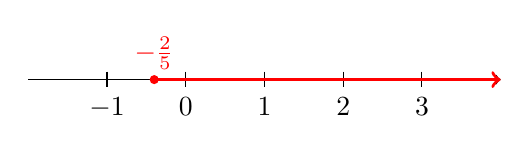
\begin{tikzpicture}
        \draw[->] (-2,0)--(4,0); 
        % routine for ticks
        %\draw (-2,+0.1) -- (-2,-0.1) node[below] {$-2$};
        \draw (-1,+0.1) -- (-1,-0.1) node[below] {$-1$};
        \draw (0,+0.1) -- (0,-0.1) node[below] {$0$};
        \draw (1,+0.1) -- (1,-0.1) node[below] {$1$};
        \draw (2,+0.1) -- (2,-0.1) node[below] {$2$};
        \draw (3,+0.1) -- (3,-0.1) node[below] {$3$};
        %\draw (4,+0.1) -- (4,-0.1) node[below] {$4$};
        \draw[very thick,color=red,->] (-0.4,0)--(4,0);
        \draw[color=red,fill=red] (-0.4,0) circle(0.05cm) 
          node[above] {$-\frac{2}{5}$} ;
        %\draw[color=red,fill=red] (0,0)    circle(0.05cm) ;
      \end{tikzpicture}
      \caption{Graph of the solution set of $6-5x\le 8$}
      \label{fig:6-5x}
    \end{figure}
  \item $3x-1<2-x \implies 4x < 3 \implies x < \frac{3}{4}$.  See
    Figure~\ref{fig:3x-1LT2-x}.  (Alternatively you could have move
    the $x$'s to the RHS: $\ds 3x-1<2-x \implies -3 < -4x$, and at
    this point you must remember to switch the direction of the
    inequality sign when you divide through by $-4$.  It is best to
    avoid altogether the possibility of making an error by initially
    moving the $x$'s to whichever side makes the coefficient positive,
    as in the first method.)
    %Figure~\ref{fig:3x-1LT2-x}. 
    \begin{figure}[htbp]
      \centering
      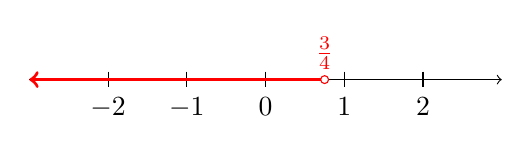
\begin{tikzpicture}
        \draw[->] (-3,0)--(3,0); 
        % routine for ticks
        \draw (-2,+0.1) -- (-2,-0.1) node[below] {$-2$};
        \draw (-1,+0.1) -- (-1,-0.1) node[below] {$-1$};
        \draw (0,+0.1) -- (0,-0.1) node[below] {$0$};
        \draw (1,+0.1) -- (1,-0.1) node[below] {$1$};
        \draw (2,+0.1) -- (2,-0.1) node[below] {$2$};
        %\draw (3,+0.1) -- (3,-0.1) node[below] {$3$};
        %\draw (4,+0.1) -- (4,-0.1) node[below] {$4$};
        \draw[very thick,color=red,<-] (-3,0)--(0.75,0); % 0.75=3/4
        \draw[color=red,fill=white] (0.75,0) circle(0.05cm) 
          node[above] {$\frac{3}{4}$} ;
        %\draw[color=red,fill=red] (0,0)    circle(0.05cm) ;
      \end{tikzpicture}
      \caption{Graph of the solution set of $3x-1<2-x$}
      \label{fig:3x-1LT2-x}
    \end{figure}
  \item % $\ds -2\le 3-2x\le 6$
    This is really two inequalities.  In general, we solve two
    inequalities separately, but in this case we can solve them
    simultaneously.  Adding $-3$ everywhere we have
    \begin{equation*}
      -5 \le -2x \le 3
    \end{equation*}
    Dividing through by $-2$ and \textit{reversing the sign of the
      inequalities} we have
    \begin{equation*}
      \frac{5}{2} \ge x \ge -\frac{3}{2}
    \end{equation*}
    which I prefer to write using the $\le$ symbol:
    \begin{equation*}
      -\frac{3}{2} \le x \le \frac{5}{2}
    \end{equation*}
    See Figure~\ref{fig:-2LE3-2xLE6}. 
    \begin{figure}[htbp]
      \centering
      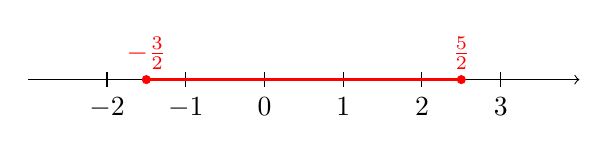
\begin{tikzpicture}
        \draw[->] (-3,0)--(4,0); 
        % routine for ticks
        %\draw (-2,+0.1) -- (-2,-0.1) node[below] {$-2$};
        \draw (-2,+0.1) -- (-2,-0.1) node[below] {$-2$};
        \draw (-1,+0.1) -- (-1,-0.1) node[below] {$-1$};
        \draw (0,+0.1) -- (0,-0.1) node[below] {$0$};
        \draw (1,+0.1) -- (1,-0.1) node[below] {$1$};
        \draw (2,+0.1) -- (2,-0.1) node[below] {$2$};
        \draw (3,+0.1) -- (3,-0.1) node[below] {$3$};
        %\draw (4,+0.1) -- (4,-0.1) node[below] {$4$};
        \draw[very thick,color=red,-] (-1.5,0)--(2.5,0); % 0.75=3/4
        \draw[color=red,fill=red] (-1.5,0) circle(0.05cm) 
          node[above] {$-\frac{3}{2}$} ;
        \draw[color=red,fill=red]   (2.5,0) circle(0.05cm)
          node[above] {$\frac{5}{2}$} ;
      \end{tikzpicture}
      \caption{Graph of the solution set of $-2\le 3-2x\le 6$}
      \label{fig:-2LE3-2xLE6}
    \end{figure}
  \end{enumerate}
\item % (Based on A.43--44) Solve the equation for $x$.
  \begin{enumerate}
  \item $\ds |4x|=1$ means ``$\ds 4x=-1$ or $\ds 4x=1$''.  In the
    first case, we have $x=-\frac{1}{4}$.  In the second case, we have
    $x=\frac{1}{4}$.  Altogether, the solution set is
    $\{-\frac{1}{4},\frac{1}{4}\}$.  You should check that each number
    in the set really is a solution to the given equation.
  \item $|2x-1|=4$ means $2x-1=-4$ or $2x-1=4$.  In the first case, we
    have $2x=-3$, $x=-\frac{3}{2}$.  In the second case, we have
    $2x=5$, $x=\frac{5}{2}$.  Altogether the solution set is
    $\{-\frac{3}{2},\frac{5}{2}\}$.  You should check that each number
    in the solution set really is a solution to the given equation.
  \end{enumerate}
\item % (Based on A.47--54) Solve the inequality.
  \begin{enumerate}
  \item $|x|\ge 5$ means $x\le -5$ or $5\le x$.  See
    Figure~\ref{fig:abs-x-ge-5}.
    \begin{figure}[htbp]
      \centering
      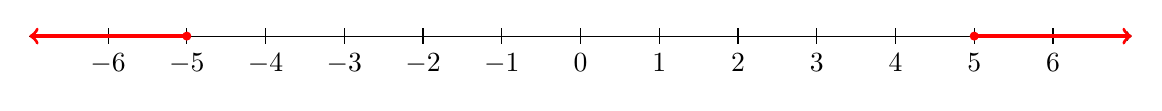
\begin{tikzpicture}
        \draw[->] (-7,0)--(7,0); 
        % routine for ticks
        \draw (-6,+0.1) -- (-6,-0.1) node[below] {$-6$};
        \draw (-5,+0.1) -- (-5,-0.1) node[below] {$-5$};
        \draw (-4,+0.1) -- (-4,-0.1) node[below] {$-4$};
        \draw (-3,+0.1) -- (-3,-0.1) node[below] {$-3$};
        \draw (-2,+0.1) -- (-2,-0.1) node[below] {$-2$};
        \draw (-1,+0.1) -- (-1,-0.1) node[below] {$-1$};
        \draw (0,+0.1) -- (0,-0.1) node[below] {$0$};
        \draw (1,+0.1) -- (1,-0.1) node[below] {$1$};
        \draw (2,+0.1) -- (2,-0.1) node[below] {$2$};
        \draw (3,+0.1) -- (3,-0.1) node[below] {$3$};
        \draw (4,+0.1) -- (4,-0.1) node[below] {$4$};
        \draw (5,+0.1) -- (5,-0.1) node[below] {$5$};
        \draw (6,+0.1) -- (6,-0.1) node[below] {$6$};
        \draw[very thick,color=red,->] (-5,0)--(-7,0);
        \draw[very thick,color=red,->] (5,0)--(7,0); 
        \draw[color=red,fill=red] (-5,0) circle(0.05cm) ;
        %  node[above] {$-\frac{3}{2}$} ;
        \draw[color=red,fill=red] (5,0) circle(0.05cm) ;
        %  node[above] {$\frac{5}{2}$} ;
      \end{tikzpicture}
      \caption{Graph of the solution set of $|x|\ge 5$}
      \label{fig:abs-x-ge-5}
    \end{figure}
  \item $|x-2|\le 0.5$ means
    \begin{equation*}
      -0.5 \le x-2 \le 0.5
    \end{equation*}
    Solving the two inequalities simultaneously by adding $2$ everywhere,
    \begin{equation*}
      1.5 \le x \le 2.5
    \end{equation*}
    See Figure~\ref{fig:abs-x-minus-2-le-0.5}.
    \begin{figure}[htbp]
      \centering
      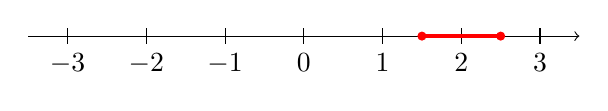
\begin{tikzpicture}
        \draw[->] (-3.5,0)--(3.5,0); 
        % routine for ticks
        %\draw (-6,+0.1) -- (-6,-0.1) node[below] {$-6$};
        %\draw (-5,+0.1) -- (-5,-0.1) node[below] {$-5$};
        %\draw (-4,+0.1) -- (-4,-0.1) node[below] {$-4$};
        \draw (-3,+0.1) -- (-3,-0.1) node[below] {$-3$};
        \draw (-2,+0.1) -- (-2,-0.1) node[below] {$-2$};
        \draw (-1,+0.1) -- (-1,-0.1) node[below] {$-1$};
        \draw (0,+0.1) -- (0,-0.1) node[below] {$0$};
        \draw (1,+0.1) -- (1,-0.1) node[below] {$1$};
        \draw (2,+0.1) -- (2,-0.1) node[below] {$2$};
        \draw (3,+0.1) -- (3,-0.1) node[below] {$3$};
        %\draw (4,+0.1) -- (4,-0.1) node[below] {$4$};
        %\draw (5,+0.1) -- (5,-0.1) node[below] {$5$};
        %\draw (6,+0.1) -- (6,-0.1) node[below] {$6$};
        \draw[very thick,color=red,-] (1.5,0)--(2.5,0);
        %\draw[very thick,color=red,->] (5,0)--(7,0); 
        \draw[color=red,fill=red] (1.5,0) circle(0.05cm) ;
        %  node[above] {$-\frac{3}{2}$} ;
        \draw[color=red,fill=red] (2.5,0) circle(0.05cm) ;
        %  node[above] {$\frac{5}{2}$} ;
      \end{tikzpicture}
      \caption{Graph of the solution set of $|x-2|\le 0.5$}
      \label{fig:abs-x-minus-2-le-0.5}
    \end{figure}
  \item $\ds |x+1|\ge 2$ means $x+1 \le -2$ or $\ds 2\le x+1$.
    Solving the two inequalities simultaneously by subtracting $1$
    everywhere, $x\le -3$ or $1\le x$.  See
    Figure~\ref{fig:abs-x-plus-1-ge-2}.
    \begin{figure}[htbp]
      \centering
      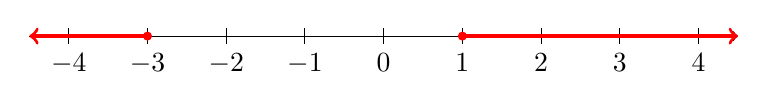
\begin{tikzpicture}
        \draw[->] (-4.5,0)--(4.5,0); 
        % routine for ticks
        %\draw (-6,+0.1) -- (-6,-0.1) node[below] {$-6$};
        %\draw (-5,+0.1) -- (-5,-0.1) node[below] {$-5$};
        \draw (-4,+0.1) -- (-4,-0.1) node[below] {$-4$};
        \draw (-3,+0.1) -- (-3,-0.1) node[below] {$-3$};
        \draw (-2,+0.1) -- (-2,-0.1) node[below] {$-2$};
        \draw (-1,+0.1) -- (-1,-0.1) node[below] {$-1$};
        \draw (0,+0.1) -- (0,-0.1) node[below] {$0$};
        \draw (1,+0.1) -- (1,-0.1) node[below] {$1$};
        \draw (2,+0.1) -- (2,-0.1) node[below] {$2$};
        \draw (3,+0.1) -- (3,-0.1) node[below] {$3$};
        \draw (4,+0.1) -- (4,-0.1) node[below] {$4$};
        %\draw (5,+0.1) -- (5,-0.1) node[below] {$5$};
        %\draw (6,+0.1) -- (6,-0.1) node[below] {$6$};
        \draw[very thick,color=red,->] (-3,0)--(-4.5,0);
        \draw[very thick,color=red,->] (1,0)--(4.5,0); 
        \draw[color=red,fill=red] (-3,0) circle(0.05cm) ;
        %  node[above] {$-\frac{3}{2}$} ;
        \draw[color=red,fill=red] (1,0) circle(0.05cm) ;
        %  node[above] {$\frac{5}{2}$} ;
      \end{tikzpicture}
      \caption{Graph of the solution set of $|x-2|\le 0.5$}
      \label{fig:abs-x-plus-1-ge-2}
    \end{figure}
  \item $|3x-1|<4$ means $-4<3x-1<4$.  Solving both inequalities
    simultaneously,
    \begin{equation*}
      -4<3x-1<4 \implies -3<3x<5 \implies -1<x<\frac{5}{3}
    \end{equation*}
    See Figure~\ref{fig:abs-3x-minus-1-lt-4}.
    \begin{figure}[htbp]
      \centering
      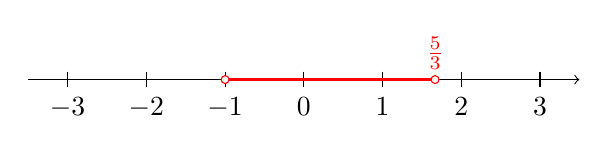
\begin{tikzpicture}
        \draw[->] (-3.5,0)--(3.5,0); 
        % routine for ticks
        %\draw (-6,+0.1) -- (-6,-0.1) node[below] {$-6$};
        %\draw (-5,+0.1) -- (-5,-0.1) node[below] {$-5$};
        %\draw (-4,+0.1) -- (-4,-0.1) node[below] {$-4$};
        \draw (-3,+0.1) -- (-3,-0.1) node[below] {$-3$};
        \draw (-2,+0.1) -- (-2,-0.1) node[below] {$-2$};
        \draw (-1,+0.1) -- (-1,-0.1) node[below] {$-1$};
        \draw (0,+0.1) -- (0,-0.1) node[below] {$0$};
        \draw (1,+0.1) -- (1,-0.1) node[below] {$1$};
        \draw (2,+0.1) -- (2,-0.1) node[below] {$2$};
        \draw (3,+0.1) -- (3,-0.1) node[below] {$3$};
        %\draw (4,+0.1) -- (4,-0.1) node[below] {$4$};
        %\draw (5,+0.1) -- (5,-0.1) node[below] {$5$};
        %\draw (6,+0.1) -- (6,-0.1) node[below] {$6$};
        \draw[very thick,color=red,-] (-1,0)--({5/3},0);
        %\draw[very thick,color=red,->] ({5/3},0)--(3.5,0); 
        \draw[color=red,fill=white] (-1,0) circle(0.05cm) ;
        %  node[above] {$-\frac{3}{2}$} ;
        \draw[color=red,fill=white] ({5/3},0) circle(0.05cm) 
        node[above] {$\frac{5}{3}$} ;
      \end{tikzpicture}
      \caption{Graph of the solution set of $|3x-1|< 4$}
      \label{fig:abs-3x-minus-1-lt-4}
    \end{figure}
  \end{enumerate}
\item % (Based on A.9--12) Rewrite the expression without using the absolute
  % value symbol.
  We could rewrite the absolute value expressions using the cases
  construction discussed in the lectures but there is a tidier way:
  \begin{enumerate}
  \item $\ds |1-2x| = \sqrt{(1-2x)^2}$
  \item $\ds |x^2-1| = \sqrt{(x^2-1)^2}$
  \end{enumerate}
\item % (Based on A.23--38) Solve the inequality in terms of intervals and
  % illustrate the solution set on the real number line.
  \begin{enumerate}
  \item % $\ds 4x-5 < 3x-2 < 5x+2$
    Since there are $x$'s in multiple locations in the given
    inequality $4x-5 < 3x-2 < 5x+2$, rather than just one $x$, we
    can't simultaneously solve both inequalities, so we must work on
    them one at a time.  Solving the first inequality,
    \begin{equation*}
      4x-5 < 3x-2 \implies x < 3
    \end{equation*}
    Solving the second inequality,
    \begin{equation*}
      3x-2 < 5x+2 \implies -4<2x \implies -2<x
    \end{equation*}
    (note how I avoided having to divide through by a negative number
    by carefully chosing which side of the inequality to put my
    $x$'s).  Recombining the results, we have the solution $-2<x<3$.
    See Figure~\ref{fig:4x-5LT3x-2LT5x+2}. 
    \begin{figure}[htbp]
      \centering
      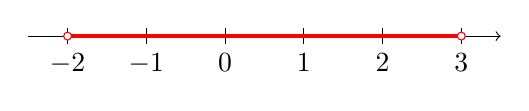
\begin{tikzpicture}
        \draw[->] (-2.5,0)--(3.5,0); 
        % routine for ticks
        \draw (-2,+0.1) -- (-2,-0.1) node[below] {$-2$};
        \draw (-1,+0.1) -- (-1,-0.1) node[below] {$-1$};
        \draw (0,+0.1) -- (0,-0.1) node[below] {$0$};
        \draw (1,+0.1) -- (1,-0.1) node[below] {$1$};
        \draw (2,+0.1) -- (2,-0.1) node[below] {$2$};
        \draw (3,+0.1) -- (3,-0.1) node[below] {$3$};
        %\draw (4,+0.1) -- (4,-0.1) node[below] {$4$};
        \draw[very thick,color=red,-] (-2,0)--(3,0); 
        \draw[color=red,fill=white] (-2,0) circle(0.05cm) ;
          %node[above] {%$\frac{1}{2}$} ;
        \draw[color=red,fill=white]   (3,0) circle(0.05cm) ;
          %node[above] {$\frac{5}{2}$} ;
      \end{tikzpicture}
      \caption{Graph of the solution set of $4x-5<3x-2<5x+2$}
      \label{fig:4x-5LT3x-2LT5x+2}
    \end{figure}
  \item % $3x^2-x-4 \ge 0$
    In this case we factor the quadratic to obtain
    \begin{equation*}
      (x+1)(3x-4) \ge 0
    \end{equation*}
    Note that I have ordered the factors by increasing root: the root
    of $x+1$ is $x=-1$, and the root of $3x-4$ is $x=\frac{4}{3}$.  We
    now develop a table as discussed in the lectures; see
    Table~\ref{tab:px+1pp3x-4p}.
    \begin{table}[htbp]
      \centering
      \begin{tabular}{|ccccc|c|c|c|}
        \hline
        \multicolumn{5}{|c|}{$I$} & $(x+1)$ & $(3x-4)$ & $(x+1)(3x-4)$ \\
        \hline\hline
        $   $&$ $&$x$&$  <$&$ -1$  & $-$     & $-$      & $+$           \\
        \hline
        $   $&$ $&$x$&$  =$&$ -1$  & $0$     & $-$      & $0$           \\
        \hline
        $ -1$&$<$&$x$&$  <$&$3/4$  & $+$     & $-$      & $-$           \\
        \hline
        $   $&$ $&$x$&$  =$&$3/4$  & $+$     & $0$      & $0$           \\
        \hline
        $3/4$&$<$&$x$&$   $&$   $  & $+$     & $+$      & $+$           \\
        \hline
      \end{tabular}
      \caption{Determining the sign of $(x+1)(3x-4)$}
      \label{tab:px+1pp3x-4p}
    \end{table}
    From the last column of the table it follows that the cases in
    which $(x+1)(3x-4)\ge 0$ are $x<-1$, $x=-1$, $x=\frac{3}{4}$, or
    $\frac{3}{4}<x$.  We can combine those possibilities into a two
    inequalities describing the solution set: ``$x\le-1$ or
    $\frac{3}{4}\le x$''.  See Figure~\ref{fig:3x2-x-4GE0}.
    \begin{figure}[htbp]
      \centering
      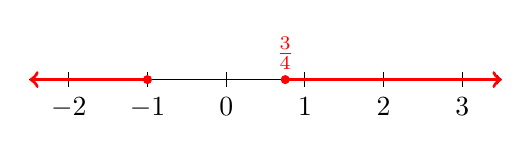
\begin{tikzpicture}
        \draw[->] (-2.5,0)--(3.5,0); 
        % routine for ticks
        \draw (-2,+0.1) -- (-2,-0.1) node[below] {$-2$};
        \draw (-1,+0.1) -- (-1,-0.1) node[below] {$-1$};
        \draw (0,+0.1) -- (0,-0.1) node[below] {$0$};
        \draw (1,+0.1) -- (1,-0.1) node[below] {$1$};
        \draw (2,+0.1) -- (2,-0.1) node[below] {$2$};
        \draw (3,+0.1) -- (3,-0.1) node[below] {$3$};
        %\draw (4,+0.1) -- (4,-0.1) node[below] {$4$};
        \draw[very thick,color=red,<-] (-2.5,0)--(-1,0); 
        \draw[color=red,fill=red] (-1,0) circle(0.05cm)
          %node[above] {%$\frac{1}{2}$}
          ;
        \draw[very thick,color=red,->] (0.75,0)--(3.5,0); 
        \draw[color=red,fill=red]   (0.75,0) circle(0.05cm)
          node[above] {$\frac{3}{4}$} 
          ;
      \end{tikzpicture}
      \caption{Graph of the solution set of $3x^2-x-4\ge 0$}
      \label{fig:3x2-x-4GE0}
    \end{figure}
  \item % $\ds x^3+6x<5x^2$
    First, we move everything to the LHS leaving just $0$ in the RHS:
    \begin{equation*}
      x^3-5x^2+6x < 0
    \end{equation*}
    Next, we attempt to factor the cubic.  There is a common factor of
    $x$ in every term so we take that out:
    \begin{equation*}
      x(x^2-5x+6) < 0
    \end{equation*}
    Now we factor the quadratic:
    \begin{equation*}
      x(x-2)(x-3) < 0
    \end{equation*}
    Note that the factors are written in order of increasing root.  In
    order to determine the sign of the LHS we build
    Table~\ref{tab:xpx-2ppx-3p}.
    \begin{table}[htbp]
      \centering
      \begin{tabular}{|ccccc||c|c|c||c|}
        \hline
        \multicolumn{5}{|c||}{$I$} & $x$ & $(x-2)$ & $(x-3)$ & $x(x-2)(x-3)$ \\
        \hline\hline
        $  $&$  $&$ x$&$ <$&$ 0$   & $-$ & $-$     & $-$     & $-$           \\
        \hline
        $  $&$  $&$ x$&$ =$&$ 0$   & $0$ & $-$     & $-$     & $0$           \\
        \hline
        $ 0$&$ <$&$ x$&$ <$&$ 2$   & $+$ & $-$     & $-$     & $+$           \\
        \hline
        $  $&$  $&$ x$&$ =$&$ 2$   & $+$ & $0$     & $-$     & $0$           \\
        \hline
        $ 2$&$ <$&$ x$&$ <$&$ 3$   & $+$ & $+$     & $-$     & $-$           \\
        \hline
        $  $&$  $&$ x$&$ =$&$ 3$   & $+$ & $+$     & $0$     & $0$           \\
        \hline
        $ 3$&$ <$&$ x$&$  $&$  $   & $+$ & $+$     & $+$     & $+$           \\
        \hline
      \end{tabular}
      \caption{Determining the sign of $x(x-2)(x-3)$}
      \label{tab:xpx-2ppx-3p}
    \end{table}
    From the last column of the table, we see that $x(x-2)(x-3)<0$
    when $x<0$ or when $2<x<3$, which is the solution set for our
    inequality.  See Figure~\ref{fig:x3+6xLT5x2}.
    \begin{figure}[htbp]
      \centering
      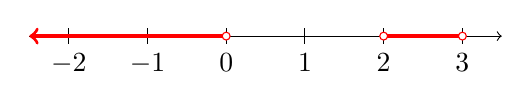
\begin{tikzpicture}
        \draw[->] (-2.5,0)--(3.5,0); 
        % routine for ticks
        \draw (-2,+0.1) -- (-2,-0.1) node[below] {$-2$};
        \draw (-1,+0.1) -- (-1,-0.1) node[below] {$-1$};
        \draw (0,+0.1) -- (0,-0.1) node[below] {$0$};
        \draw (1,+0.1) -- (1,-0.1) node[below] {$1$};
        \draw (2,+0.1) -- (2,-0.1) node[below] {$2$};
        \draw (3,+0.1) -- (3,-0.1) node[below] {$3$};
        %\draw (4,+0.1) -- (4,-0.1) node[below] {$4$};
        \draw[very thick,color=red,<-] (-2.5,0)--(0,0); 
        \draw[color=red,fill=white] (0,0) circle(0.05cm)
          %node[above] {%$\frac{1}{2}$}
          ;
        \draw[very thick,color=red,-] (2,0)--(3,0); 
        \draw[color=red,fill=white]   (2,0) circle(0.05cm)
          %node[above] {$\frac{3}{4}$} 
          ;
        \draw[color=red,fill=white]   (3,0) circle(0.05cm)
          %node[above] {$\frac{3}{4}$} 
          ;
      \end{tikzpicture}
      \caption{Graph of the solution set of $x^3+6x<5x^2$}
      \label{fig:x3+6xLT5x2}
    \end{figure}
  \item % $-1<1/x\le 3$
    This problem is rather tricky.  The temptation is to multiply by
    $x$, but remember that if
    $x$ is negative, we must reverse the direction of the inequality
    signs.  The problem is that we don't know anything about
    $x$; it could be positive \textit{or} negative.

    One way out of this is to make a series of assumptions that cover
    all the cases.  The assumptions provide a context within which we
    can make progress.  We are going to look at the cases
    $x<0$, $x=0$, and $x>0$ which cover all the possibilities for
    $x$.  We can quickly dispense with the case $x=0$ because
    $1/x$ is not defined for $x=0$.

    Next let us assume that $x<0$.  Then $1/x\le 3$ is automatically
    satisfied because $1/x < 0 < 3$.  To solve $-1<1/x$ we multiply
    both sides by the negative number $x$ \textit{and reverse the sign
      of the inequality} to obtain $-x>1$.  We multiply both sides by
    $-1$ and reverse the inequality sign a second time to obtain
    $x<-1$.

    Conversely, if $x<-1$ then $x<0$ for sure, so $1/x<0<3$, so
    $1/x\le 3$ is satisfied; and we obtain $-1<1/x$ by dividing $x<-1$
    through by $-x$ (which is a positive number).

    Finally let us assume that $0<x$.  Then $-1<1/x$ is automatically
    satisfied because $-1<0<1/x$, and we just have to ensure
    $1/x\le 3$.  Because $x>0$ we can apply the reciprocal rule, and
    so we have $\frac{1}{3}\le x$.

    Conversely, if $\frac{1}{3}\le x$, then $0<x$ so we can apply the
    reciprocal rule to obtain $1/x\le 3$ and we also have $-1<1/x$
    because $-1<0<1/x$, so the inequality $-1<1/x\le 3$ is satisfied.

    In summary, the inequality $-1<1/x\le 3$ is satisfied when $x<-1$
    or when $\frac{1}{3}\le x$.  See Figure~\ref{fig:-1LT1oxLE3}.
    \begin{figure}[htbp]
      \centering
      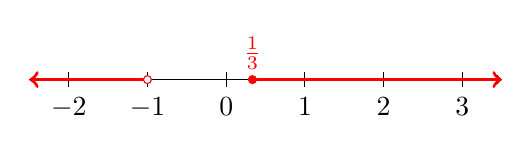
\begin{tikzpicture}
        \draw[->] (-2.5,0)--(3.5,0); 
        % routine for ticks
        \draw (-2,+0.1) -- (-2,-0.1) node[below] {$-2$};
        \draw (-1,+0.1) -- (-1,-0.1) node[below] {$-1$};
        \draw (0,+0.1) -- (0,-0.1) node[below] {$0$};
        \draw (1,+0.1) -- (1,-0.1) node[below] {$1$};
        \draw (2,+0.1) -- (2,-0.1) node[below] {$2$};
        \draw (3,+0.1) -- (3,-0.1) node[below] {$3$};
        %\draw (4,+0.1) -- (4,-0.1) node[below] {$4$};
        \draw[very thick,color=red,<-] (-2.5,0)--(-1,0); 
        \draw[color=red,fill=white] (-1,0) circle(0.05cm)
          %node[above] {%$\frac{1}{2}$}
          ;
        \draw[very thick,color=red,->] (1/3,0)--(3.5,0); 
        \draw[color=red,fill=red]   (1/3,0) circle(0.05cm)
          node[above] {$\frac{1}{3}$} 
          ;
        %\draw[color=red,fill=white]   (3,0) circle(0.05cm)
        %  %node[above] {$\frac{3}{4}$} 
        %  ;
      \end{tikzpicture}
      \caption{Graph of the solution set of $-1<1/x\le 3$}
      \label{fig:-1LT1oxLE3}
    \end{figure}
    We will learn another way to solve this type of problem later in
    the course.
  \end{enumerate}
\item % (Based on A.39--42) As dry air moves upward, it expands and in so
  % doing cools at a rate of about $1^{\circ}$C for each 100 m rise, up to
  % about 12000 m.  
  \begin{enumerate}
  \item % If the ground temperature is $20^{\circ}$C, write a formula for the
    % temperature at height $h$.
    The temperature $T$ in degrees Celsius at height $h$ in meters is given by
    \begin{equation*}
      \mbox{$\ds T = 20 - \frac{1}{100}h$, $0\le h \le 12000$}
    \end{equation*}
    That says we start with a temperature of 20, then
    \textit{decrease} ($-$) at a \textit{rate of 1 degree per 100}
    ($\frac{1}{100}$) meters ($h$).  We also note that the formula is
    only applicable above the ground ($h\ge 0$) and below a height of
    about 12000 meters ($h\le 12000$).
  \item % What range of temperature can be expected if a plane takes
        % off and reaches standard cruising altitude of 11 000 m?  XX
    We know that $0\le h \le 11000$ in this part of the problem, and
    we want to find an inequality for $T$.  We modify the inequality
    for $h$ until the expression in the middle looks more like $T$.
    First we multiply throughout by $-\frac{1}{100}$:
    \begin{equation*}
      0 \le h \le 11000 \implies 0 \ge -\frac{1}{100} h \ge -110
    \end{equation*}
    Note that we have reversed the sign of the inequalities because
    $-\frac{1}{100}$ is negative.  Now we add 20 throughout:
    \begin{equation*}
      -110 \le -\frac{1}{100} h \le 0 
      \implies -90 \le 20 - \frac{1}{100} h \le 20
    \end{equation*}
    So the range of temperatures we can expect on such a flight is 
    \begin{equation*}
      -90 \le T \le 20
    \end{equation*}
  \end{enumerate}
\item % (Based on A.45--46) Solve the equation for $x$.
  \begin{enumerate}
  \item % $\ds \frac{|2x+1|}{|x-1|}=3$
    There are two sets of absolute value symbols in the problem.  We
    can reduce the number of absolute value symbols as follows.  We
    have
    \begin{equation*}
      \frac{|2x+1|}{|x-1|} = 3
      \implies \left| \frac{2x+1}{x-1} \right| = 3
      \implies \mbox{$\ds \frac{2x+1}{x-1} = -3$ 
        or $\ds \frac{2x+1}{x-1} = 3$}
    \end{equation*}
    In the first case we have
    \begin{equation*}
      \frac{2x+1}{x-1} = -3 \implies 2x+1 = -3(x-1)
      \implies 2x+1 = -3x + 3 \implies 5x = 2 \implies x=\frac{2}{5}
    \end{equation*}
    In the second case we have
    \begin{equation*}
      \frac{2x+1}{x-1} = 3 \implies 2x+1 = 3(x-1) 
      \implies 2x+1 = 3x-3 \implies 4 = x
    \end{equation*}
    So our solution set is $\{\frac{2}{5},4\}$.  You should check that
    both of those numbers satisfy the original problem.
  \item % $\ds \vphantom{\frac{|x|}{|x|}} |x+4| = |3x-2|$
    Solving this problem benefits from some creative thinking.  One
    way to do it might be to break it up into four cases, e.g.,
    $x+4<0$ and $3x-2<0$ would be one case.  Another way would be to
    break the line up into five pieces ($x<-4$, $x=-4$,
    $-4<x<\frac{2}{3}$, $x=\frac{2}{3}$, $\frac{2}{3}<x$) like we did
    when solving inequalities with quadratics.  However, in this case
    I recommend dividing both sides of the equation by $|x+4|$.  In
    order to do so, we must first check that $x=-4$ is not a solution
    to the equation (it is not) so we know that $|x+4|\ne 0$ and we
    can divide through by $|x+4|$:
    \begin{equation*}
      1 = \frac{|3x-2|}{|x+4|} 
      \implies 1 = \left| \frac{3x-2}{x+4} \right|
    \end{equation*}
    where we have used the absolute value rule
    $|a|/|b|=|a/b|$ as in the previous problem.  Now there is only one
    absolute value sign in the expression and we can use the usual
    method for solving absolute value equalities.  We have
    \begin{equation*}
      \left| \frac{3x-2}{x+4} \right| = 1
      \Longleftrightarrow 
      \mbox{$\ds \frac{3x-2}{x+4} = -1$ or $\ds \frac{3x-2}{x+4} = 1$}
    \end{equation*}
    In the first case we have 
    \begin{equation*}
      \frac{3x-2}{x+4} = -1 \implies 3x-2 = -(x+4) \implies
      3x-2 = -x-4 \implies 4x = -2 \implies x = -\frac{1}{2}
    \end{equation*}
    In the second case we have
    \begin{equation*}
      \frac{3x-2}{x+4} = 1 \implies 3x-2 = x+4 \implies 2x = 6
      \implies x=3
    \end{equation*}
    So the solution set is $\{-\frac{1}{2},3\}$.  You should check
    that both of those numbers actually are solutions to the equation.
  \end{enumerate}
\item % (Based on A.55--56)
  \begin{enumerate}
  \item % $\ds 3\le |2x| \le 5$
    The most straightforward way to see this is to consider the cases
    $2x< 0$, $2x=0$, and $2x>0$ separately.  The case
    $2x=0$ is obviously eliminated because it implies
    $x=0$ which clearly does not satisfy the inequality.

    In the first case, $2x<0$ implies that
    $|2x|=-2x$ by the definition of absolute value so the inequality
    becomes
    \begin{equation*}
      3\le -2x \le 5 \implies -\frac{3}{2} \ge x \ge -\frac{5}{2}
      \implies -\frac{5}{2} \le x \le -\frac{3}{2}
    \end{equation*}
    where I have just re-written the last inequality using my
    preference of $\le$ over
    $\ge$.  You should check that conversely, $-\frac{5}{2} \le x \le
    -\frac{3}{2}$ implies that $3\le |2x| \le 5$.

    In the remaining case, $2x> 0$ implies that
    $|2x|=2x$ so the inequality becomes
    \begin{equation*}
      3\le 2x \le 5 \implies \frac{3}{2} \le x \le \frac{5}{2} 
    \end{equation*}
    You should check that conversely, $\frac{3}{2} \le x \le
    \frac{5}{2}$ implies that $3\le |2x| \le 5$.
    
    In summary, the solution set is $x$ either in the interval
    $[-\frac{5}{2},-\frac{3}{2}]$ or in the interval
    $[\frac{3}{2},\frac{5}{2}]$.  In other words, the solution set is
    the union
    $[-\frac{5}{2},-\frac{3}{2}]\cup [\frac{3}{2},\frac{5}{2}]$.  See
    Figure~\ref{fig:3LEabs2xLE5}.
    \begin{figure}[htbp]
      \centering
      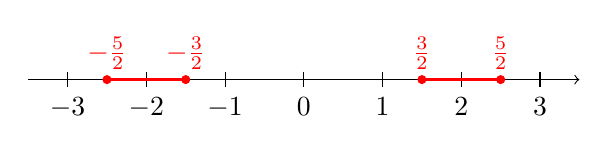
\begin{tikzpicture}
        \draw[->] (-3.5,0)--(3.5,0); 
        % routine for ticks
        \draw (-3,+0.1) -- (-3,-0.1) node[below] {$-3$};
        \draw (-2,+0.1) -- (-2,-0.1) node[below] {$-2$};
        \draw (-1,+0.1) -- (-1,-0.1) node[below] {$-1$};
        \draw (0,+0.1) -- (0,-0.1) node[below] {$0$};
        \draw (1,+0.1) -- (1,-0.1) node[below] {$1$};
        \draw (2,+0.1) -- (2,-0.1) node[below] {$2$};
        \draw (3,+0.1) -- (3,-0.1) node[below] {$3$};
        %\draw (4,+0.1) -- (4,-0.1) node[below] {$4$};
        \draw[very thick,color=red,-] (-2.5,0)--(-1.5,0); 
        \draw[color=red,fill=red] (-2.5,0) circle(0.05cm)
          node[above] {$-\frac{5}{2}$}
          ;
        \draw[color=red,fill=red] (-1.5,0) circle(0.05cm)
          node[above] {$-\frac{3}{2}$}
          ;
        \draw[very thick,color=red,-] (1.5,0)--(2.5,0); 
        \draw[color=red,fill=red]   (1.5,0) circle(0.05cm)
          node[above] {$\frac{3}{2}$} 
          ;
        \draw[color=red,fill=red]   (2.5,0) circle(0.05cm)
          node[above] {$\frac{5}{2}$} 
          ;
      \end{tikzpicture}
      \caption{Graph of the solution set of $3\le |2x| \le 5$}
      \label{fig:3LEabs2xLE5}
    \end{figure}  
  \item % $\ds 0<|x-4|<1$
    This problem is similar to the previous, but the outcome is
    slightly different.  We again consider two separate cases, $x-4\ge
    0$ and $x-4<0$.  In the first case we have
    \begin{equation*}
      0 < |x-4| < 1 \implies 0 < x-4 < 1 \implies 4<x<5
    \end{equation*}
    In the second case we have $|x-4| = -(x-4)$ and so
    \begin{equation*}
      0 < |x-4| < 1 \implies 0 < -(x-4) < 1 \implies 0>x-4>-1 
      \implies 4>x>3 \implies 3<x<4
    \end{equation*}
    Altogether we have $x$ must satisfy $3<x<4$ or $4<x<5$.  Note that
    $x$ cannot equal 4 in either case.  See Figure~\ref{fig:0LTabsx-4LT1}.
    \begin{figure}[htbp]
      \centering
      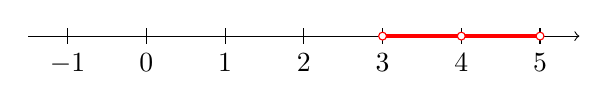
\begin{tikzpicture}
        \draw[->] (-1.5,0)--(5.5,0); 
        % routine for ticks
        %\draw (-3,+0.1) -- (-3,-0.1) node[below] {$-3$};
        %\draw (-2,+0.1) -- (-2,-0.1) node[below] {$-2$};
        \draw (-1,+0.1) -- (-1,-0.1) node[below] {$-1$};
        \draw (0,+0.1) -- (0,-0.1) node[below] {$0$};
        \draw (1,+0.1) -- (1,-0.1) node[below] {$1$};
        \draw (2,+0.1) -- (2,-0.1) node[below] {$2$};
        \draw (3,+0.1) -- (3,-0.1) node[below] {$3$};
        \draw (4,+0.1) -- (4,-0.1) node[below] {$4$};
        \draw (5,+0.1) -- (5,-0.1) node[below] {$5$};
        \draw[very thick,color=red,-] (3,0)--(5,0); 
        \draw[color=red,fill=white] (3,0) circle(0.05cm)
          %node[above] {$-\frac{5}{2}$}
          ;
        \draw[color=red,fill=white] (4,0) circle(0.05cm)
          %node[above] {$-\frac{3}{2}$}
          ;
        %\draw[very thick,color=red,-] (1.5,0)--(2.5,0); 
        \draw[color=red,fill=white]   (5,0) circle(0.05cm)
          %node[above] {$\frac{3}{2}$} 
          ;
        %\draw[color=red,fill=red]   (2.5,0) circle(0.05cm)
        %  node[above] {$\frac{5}{2}$} 
        %  ;
      \end{tikzpicture}
      \caption{Graph of the solution set of $0\le |x-4| \le 1$}
      \label{fig:0LTabsx-4LT1}
    \end{figure}
    The solution set is the interval $(3,5)$ with the point $4$
    removed from it; such a solution set is known as a
    \textit{punctured interval}.
  \end{enumerate}
\item % (Based on A.57--70)
  % Solve for $x$, assuming that $b$ and $c$ are positive and $a$ is negative.
  \begin{enumerate}
  \item % $ax+b<c$
    It doesn't matter whether $b$ is positive or negative, we can
    subtract $b$ from both sides of the inequality in either case
    without changing the direction of the inequality, so we have  
    \begin{equation*}
      ax+b < c \implies ax < c-b
    \end{equation*}
    Now, because we know that $a$ is negative, we can divide both
    sides of the inequality by $a$ provided we switch the direction of
    the inequality sign:
    \begin{equation*}
      ax < c-b \implies x > \frac{c-b}{a}
    \end{equation*}
    which is the solution to the original inequality.
  \item % $c(ax+b)\le b$
    We solve this problem in a similar manner to the previous:
    \begin{equation*}
      c(ax+b) \le b \implies ax+b \le \frac{b}{c}
      \implies ax \le \frac{b}{c} - b
      \implies x \ge \frac{1}{a} \left(\frac{b}{c} - b\right)
      \implies x \ge \frac{b}{ac} - \frac{b}{a}
    \end{equation*}
    where the last simplification was optional.  You could also add
    fractions if you wanted.
  \end{enumerate}
\item % (Based on Algebra.109--116) State whether or not the equation is true
  % for all values of the variable $x$.
  \begin{enumerate}
  \item % $\ds\vphantom{\frac{x}{x+y}}\sqrt{x^2+9}=|x|+3$
    Just try some numbers for $x$ with the assistance of your
    calculator.  If you're lucky or pick your numbers carefully, you
    don't even need a calculator.  Let's try $x=4$.  Then the LHS is
    \begin{equation*}
      \sqrt{x^2+9} = \sqrt{4^2+9} = \sqrt{16+9} = \sqrt{25} = 5
    \end{equation*}
    while the RHS is
    \begin{equation*}
      |4|+3 = 4+3 = 7
    \end{equation*}
    The LHS and the RHS disagree in this case, so the equation is
    certainly not true for all values of $x$.  (By the way, this once
    again shows that $\sqrt{x^2+9} \ne \sqrt{x^2} + \sqrt{9}$.)
  \item % $\ds \frac{a}{a+x} = \frac{1}{1+x}$
    If $a=1$, the equation certainly is true for all values of
    $x$, because in that case the LHS and the RHS are exactly the
    same.  If $a$ is any other number, i.e., $a\ne
    1$ and hence $a-1\ne 0$, then we have
    \begin{equation*}
      \frac{a}{a+x} = \frac{1}{1+x}
      \implies a(1+x) = 1(a+x) \implies a + ax = a + x
      \implies (a-1)x = 0 
      \implies x = 0
    \end{equation*}
    where we are allowed to divide by $a-1$ because we're assuming
    $a\ne 1$.  So if $a\ne 1$, the original equation is true only if
    $x=0$, which means it's not true for all values of $x$.
  \end{enumerate}
\end{enumerate}
\end{document}


%%%%%%%%%%%%%%%%%%%%%%%%%%%%%%%%%%%%%%%%%%%%%%%%%%%%%%%%%%%%%%%%%%%%%%
%%% MATH110-PS00A-Solutions.tex ends here
